\documentclass{beamer}

\usepackage[T1]{fontenc}
\usepackage{inputenc}

\usepackage{xspace}
\usepackage{xcolor}
\usepackage{multirow}

\usepackage{tikz}
\usetikzlibrary{arrows,snakes,backgrounds,patterns,matrix,shapes,fit,calc,shadows,plotmarks,intersections,shapes.geometric}

\usepackage{algpseudocode}
\usepackage{algorithm}

\usepackage{amsmath}
\usepackage{listings}
\lstset{
    basicstyle=\footnotesize,
    language=Caml,
    captionpos=b,
    frame=TB,
    showstringspaces=false,
    escapeinside={<@}{@>},
}


\usetheme{Boadilla}
\usecolortheme{dolphin}
\useoutertheme{infolines}

\beamertemplatenavigationsymbolsempty
\setbeamertemplate{footline}{
    \leavevmode%
    \hbox{%
    \begin{beamercolorbox}[wd=.333333\paperwidth,ht=2.25ex,dp=1ex,center]{author in head/foot}%
        \usebeamerfont{author in head/foot}\insertshortauthor%~~\beamer@ifempty{\insertshortinstitute}{}{(\insertshortinstitute)}
    \end{beamercolorbox}%
    \begin{beamercolorbox}[wd=.333333\paperwidth,ht=2.25ex,dp=1ex,center]{title in head/foot}%
        \usebeamerfont{title in head/foot}\insertshorttitle
    \end{beamercolorbox}%
    \begin{beamercolorbox}[wd=.333333\paperwidth,ht=2.25ex,dp=1ex,right]{date in head/foot}%
        \usebeamerfont{date in head/foot}\insertshortdate{}\hspace*{2em}
        \insertframenumber{} / 23%\inserttotalframenumber
            \hspace*{2ex}
    \end{beamercolorbox}}%
    \vskip0pt%
}


\newcommand{\TODO}{{\color{red}\bf [TODO]}}
\newcommand{\cybersec}{cybersecurity\xspace}
\newcommand{\Cybersec}{Cybersecurity\xspace}
\newcommand{\aramis}{Aramis\xspace}
\newcommand{\DiH}{Diffie-Hellman\xspace}
\newcommand{\XOR}{Exclusive-Or\xspace}
\newcommand{\modbus}{MODBUS\xspace}
\newcommand{\opcua}{OPC-UA\xspace}

\graphicspath{{assets/}}
\makeatletter
    \def\input@path{{assets/}}
\makeatother


\title{Filtering and Verifying Applicative Flows in Industrial Systems}
\author[Maxime Puys]{Maxime Puys\\[.5cm]Supervisors: Marie-Laure Potet and Jean-Louis Roch}
\institute{VERIMAG, Univ. Grenoble Alpes}
\date{January 28, 2016}



\begin{document}

\begin{frame}
    \maketitle

    \begin{columns}
        \begin{column}{.2\textwidth}
            \resizebox{\textwidth}{!}{
                \includegraphics{logo_verimag}
            }
        \end{column}
        \begin{column}{.2\textwidth}
            \resizebox{\textwidth}{!}{
                \includegraphics{logo_uga}
            }
        \end{column}
        \begin{column}{.15\textwidth}
            \resizebox{\textwidth}{!}{
                \includegraphics{logo_pia}
            }
        \end{column}
    \end{columns}
\end{frame}

\begin{frame}
    \frametitle{Industrial Systems}

    \begin{columns}
        \begin{column}{.3\textwidth}
            \resizebox{\textwidth}{!}{
                \includegraphics{scada}
            }
        \end{column}
        \begin{column}{.3\textwidth}
            \resizebox{\textwidth}{!}{
                \includegraphics{plc}
            }
        \end{column}
        \begin{column}{.3\textwidth}
            \resizebox{\textwidth}{!}{
                \includegraphics{plant}
            }
        \end{column}
    \end{columns}
    
    \begin{block}{Hot topic}
        \begin{itemize}
            \item Increasing number of attacks showed in the medias since Stuxnet \cite{Lan11}.
            \item Becoming a priority for government agencies.
            \begin{itemize}
                \item LPM to ensure the security of OIVs.
                \item Publications from ANSSI, DGA, ...
            \end{itemize}
        \end{itemize}
    \end{block}
\end{frame}

\begin{frame}
    \frametitle{Disambiguation}
    
    \begin{block}{Security concepts}
        \begin{itemize}
            \item Safety = Protection against identified/natural difficulties.
            \begin{itemize}
                \item Historic industrial concern.
            \end{itemize}
            \item \Cybersec = Protection against malicious adversaries.
            \begin{itemize}
                \item Often called Security.
            \end{itemize}
        \end{itemize}
    \end{block}
    \vfill
    \begin{figure}[htb]
        \resizebox{.85\columnwidth}{!}{
            \def\rectangle{(-.5,-1.5) rectangle (4,1.75)}
\def\secondcircle{(0:5.25) ellipse (2 and 1.5)}
\def\thridcircle{(0:-1.75) ellipse (2 and 1.5)}
\def\fourthcircle{(0:1.75) ellipse (2.25 and 1)}

\begin{tikzpicture}
    \draw \rectangle node at (1.75,1.33) {Industrial systems};
    \draw \secondcircle node {\Cybersec};
    \draw \thridcircle node {Safety};
    \draw \fourthcircle node [align=center]{Industrial \\ systems \\ \cybersec};
    \begin{scope}[fill opacity=0.25]
        \fill[blue]   \rectangle;
        \fill[red]    \secondcircle;
        \fill[green]  \thridcircle;
        \fill[yellow] \fourthcircle;
    \end{scope}
\end{tikzpicture}

        }
        \vspace{-.2cm}
        \caption{Relations among security concepts}
    \end{figure}
    \vspace{-.5cm}
    \begin{itemize}
        \item Ludovic Pietre-Cambacedes' thesis: On the relationships between safety and security, Telecom ParisTech and EDF, 2010.
    \end{itemize}
\end{frame}

\begin{frame}
    \frametitle{Differences between Industrial and Business IT}
    
    \begin{itemize}
        \item Really long-term installations, hard to patch, lot of legacy hosts.
            %\vfill
        %\item Inserting a new component must not imply existing devices modification.
            %\vfill
            \vfill
        \item Security objectives are different from traditional systems:
        \begin{itemize}
            %\item For audibility reasons and sometime performance, confidentiality is often avoided.
            \item Availability, integrity, authentication and non-repudiation.% are however very important.
        \end{itemize}
            \vfill
        %\item Industrial systems usually implement safety but rarely \cybersec:
        %\begin{itemize}
        %    \item Conditional dependancy, mutual strength, antagonism and independancy.
        %\end{itemize}
        %    \vfill
        \item Messages are READ/WRITE commands to PLCs.
        \begin{itemize}
            \item Sometimes SUBSCRIPTIONS, RPCs or grouped commands.
            \item Industrial protocols: \modbus, \opcua.
        \end{itemize}
    \end{itemize}
\end{frame}

\begin{frame}
    \frametitle{\aramis Project}% 1/2}

    \begin{itemize}
        \item Architecture Robuste pour les Automates et Mat\'eriels des Infrastructures Sensibles.
        \begin{itemize}
            \item PIA: Ministry of Industry, supervised by ANSSI.
        \end{itemize}
            \vspace{1em}
        \item Partners: ATOS World Grid, SecLab, CEA-leti, PERSYVAL-Lab.
            \vspace{1em}
        \item Objective: build a transparent device to filter industrial flows.
        \begin{itemize}
            \item Communication protocols are stopped and re-created.
            \item Applicative filtering with domain specific constraints.
        \end{itemize}
        %    \vfill
        %\item Total: 4 PhD students and 2 engineers.
    \end{itemize}
    %\vfill
    \begin{figure}[htb]
        \resizebox{.8\columnwidth}{!}{
            \begin{tikzpicture}[
    arrow/.style={thick,<->,shorten >=2pt,shorten <=2pt,>=stealth},
]

    \draw[dashed] (5,-.7) rectangle (10.5,3) node at (6,2.65) {Safe zone};
    \fill[white] (4.25,.45) rectangle (5.75,1.65);

    %\draw (0,0) rectangle (3,1) node [pos=.5] {$SCADA_{3}$};
    \draw node  at (8.5,1) {\resizebox{.2\textwidth}{!}{\includegraphics{plc}}};
    %\draw (0,3) rectangle (3,4) node [pos=.5] {$SCADA_{1}$};
    
    \draw (4,.5) rectangle (6,1.5) node [pos=.5] {$Aramis$};

    \draw node at (.9,1) {\resizebox{.3\textwidth}{!}{\includegraphics{scada}}};
   
    %\draw (10,0) rectangle (13,1) node [pos=.5] {$Client$};
    %\draw (10,3) rectangle (13,4) node [pos=.5] {$Intruders$};

    %\draw[arrow,green] (3,.5) -- (5,1.5);
    \draw[arrow,green] (2.8,1) -- (3.9,1);
    %\draw[arrow,green] (3,3.5) -- (5,2.5);

    %\draw[arrow,green] (8,1.5) -- (10,.5);
    \draw[arrow,green] (6.1,1) -- (7.2,1);
    %\draw[arrow,red] (8,2.5) -- (10,3.5);
\end{tikzpicture}

        }
        \caption{Idea of \aramis}
    \end{figure}
\end{frame}

%\begin{frame}
%    \frametitle{\aramis Project 2/2}
%
%    %\vspace{-1em}
%    \begin{itemize}
%        \item \aramis device must be really hardened:
%        \begin{itemize}
%            \item Around 350 requirements (including 100 for security).
%        \end{itemize}
%        %    \vfill
%        %\item Combine security properties of the protocols with domain specific
%        %    constraints in term of flows.
%    \end{itemize}
%    %\vspace{-.5cm}
%    %\begin{itemize}
%    %    \item I will participate within three parts:
%    %    \begin{itemize}
%    %        \item Applicative filtering,
%    %        \item Security requirements
%    %        \item Certification process.
%    %    \end{itemize}
%    %\end{itemize}
%\end{frame}

\begin{frame}
    \frametitle{Scientific Objectives}
    
    Attack models and industrial domain specific protection for provable security properties.
    %Difficult to combine security properties provided by protocols with
    %domain-specific constraints.
    \vfill
    \begin{itemize}
        \item Applicative filtering
            \vfill
        \item Attack models
            \vfill
        \item Verification of Industrial Protocols
    \end{itemize}
    \vfill
    Not redo the safety.
    %\begin{block}{Applicative filtering}
    %    Considering domain-specific constraints in term of messages flow.
    %\end{block}
    %\vfill
    %\begin{block}{Attack models}
    %    Model attacks against industrial communications according to various
    %    parameters (e.g.: network architecture, attacker's objectives, security
    %    properties of protocols).
    %\end{block}
    %\vfill
    %\begin{block}{Verification of Industrial Protocols}
    %    Formal verification of the security properties claimed by industrial
    %    protocols.
    %\end{block}
\end{frame}

\section{Applicative Filtering}

\begin{frame}
    \frametitle{Table of Contents}
    
    \tableofcontents[currentsection]
\end{frame}

\begin{frame}
    \frametitle{\aramis Filter}

    \begin{figure}[htb]
        \resizebox{\columnwidth}{!}{
            \begin{tikzpicture}[
    arrow/.style={thick,->,shorten >=2pt,shorten <=2pt,>=stealth},
]
    \draw (0,0) rectangle (8,2.5) node at (4,.4) {Aramis}; % ARAMIS
    
    \draw (.5,1) rectangle (2.5,2)  node [pos=.5] {Server}; % GH
    \draw (5.5,1) rectangle (7.5,2) node [pos=.5] {Client}; % GB

    \draw[arrow,green] (-.5,.5) -- (.5,1.25); % Arrow BL
    \draw[arrow,red] (-.5,1.5) -- (.5,1.5); % Arrow ML
    \draw[arrow,red] (-.5,2.5) -- (.5,1.75); % Arrow TL

    \draw[arrow,green] (7.5,1.25) -- (8.5,.5); % Arrow BR
    \draw[arrow,red] (7.5,1.5) -- (8.5,1.5); % Arrow MR
    %\draw[arrow,red] (7.5,1.75) -- (8.5,2.5); % Arrow TR
    
    \draw (3,1) rectangle (5,2) node [pos=.5] {Filter}; % Filters

    \draw (5.5,3) rectangle (7.5,4) node [pos=.5] {Alerts};
    \draw[arrow] (5,2) -- (5.5,3);

    \draw[arrow,blue,very thick] (5,1.25) -- (5.5,1.25); % Arrow SF
    \draw[arrow,blue,very thick] (5,1.5) -- (5.5,1.5); % Arrow SF
    %\draw[arrow,blue,very thick] (5,1.75) -- (5.5,1.75); % Arrow SF

    \draw[arrow,blue,very thick] (2.5,1.25) -- (3,1.25); % Arrow FC
    \draw[arrow,blue,very thick] (2.5,1.5) -- (3,1.5); % Arrow FC
    \draw[arrow,blue,very thick] (2.5,1.75) -- (3,1.75); % Arrow FC

    \draw (3,3) rectangle (5,4) node [pos=.5,align=center] {Efficient\\Rules}; % Rules
    \draw[arrow] (4,3) -- (4,2);

    \draw (3,5) rectangle (5,6) node [pos=.5] {Generation}; % Generator
    \draw[arrow] (4,5) -- (4,4);

    \draw (5.5,5) rectangle (8.1,6) node [pos=.5,align=center] {Domain-specific\\language}; % Rules
    \draw[arrow] (5.5,5.5) -- (5,5.5);

    \draw (0,4.5) rectangle (2,6) node at (.45,5.8) {\tiny Legend:};
    \draw[arrow,blue,very thick] (.2, 5.5) -- (.7,5.5) node [anchor=west] at (.5,5.5) {\tiny Ad-hoc lang.};
    \draw[arrow,red] (.2, 5.12) -- (.7,5.12) node [anchor=west] at (.5,5.12) {\tiny Attack msg.};
    \draw[arrow,green] (.2, 4.75) -- (.7,4.75) node [anchor=west] at (.5,4.75) {\tiny Normal msg.};
    
    \begin{scope}[fill opacity=0.25]
        \draw node  at (10,1.25) {\resizebox{.2\textwidth}{!}{\includegraphics{plc}}};
        \draw node at (-2.8,1.25) {\resizebox{.3\textwidth}{!}{\includegraphics{scada}}};
    \end{scope}
\end{tikzpicture}

        }
        \caption{Zoom on the \aramis device}
    \end{figure}
    \vspace{-1.3em}
    \begin{itemize}
        \item Double proxy and firewall.
            \vfill
        \item Embedded device:
        \begin{itemize}
            \item Memory and time constraint.
            %\item No code loading (rules must be interpreted).
        \end{itemize}
    \end{itemize}
\end{frame}

%\begin{frame}
%    \frametitle{Problem Statement}
%
%    \begin{block}{Objectives}
%        {\bf Applicative filtering:} focus on the packet's payload.
%
%        Understand the semantics behind the message to allow or reject.
%    \end{block}
%    \vfill
%    \begin{itemize}
%        \item Packets are interpreted by the \aramis device:
%        \begin{itemize}
%            \item Allow to filter the meaning of the message regardless of the protocol.
%        \end{itemize}
%    \end{itemize}
%    \vfill
%    \begin{itemize}
%        \item Messages are mostly read/write commands on variables.
%    \end{itemize}
%    \vspace{-.7em}
%    \begin{table}[htb]
%        \begin{tabular}{|c|c|}
%            \hline
%            {\bf Read Command}      & {\bf Write Command}           \\
%            \hline
%            \multicolumn{2}{|c|}{User has access to the variable?}  \\
%            \hline
%            Variable can be read ?  & Variable can be written ?     \\
%            \hline
%                                    & Value to write is valid ?     \\
%            \hline
%        \end{tabular}
%        \caption{What can be filtered?}
%    \end{table}
%    \vfill
%\end{frame}

\begin{frame}
    \frametitle{Current Filters}
    
    \begin{block}{Variable whitelist}
        {\sf foo {\color{red} 1} {\color{blue} int} {\color{green!50!black} RW} {\color{cyan} SERVER {\em IP:Port}} {\color{yellow!50!black} ACCEPT\_FROM {\em IP/Mask}} {\color{orange} VALUES 0 100}}

        \medskip
        A variable belongs to a {\color{cyan} server} and can be accessed by some {\color{yellow!50!black} clients}.

        It has a {\color{red} size}, a {\color{blue} type}, different {\color{green!50!black} permissions}, and {\color{orange} valid values}.
    \end{block}
    \vfill
    \begin{block}{Kinematic filters}
        {\sf (foo == False AND bar >= 5) PREVENT (baz := False)}

        \medskip
        The filter memorizes the values of variables into $\sigma$.

        \begin{algorithmic}
            \If {$incomingMessage$ {\bf matches} $rightPredicate$}
                \If {$\sigma \vdash leftPredicate$}
                    \State $Take~action.$
                \EndIf
            \EndIf
        \end{algorithmic}
        {\bf Drawback:} Only guaranties local decision.%applicable if global view of the system.
    \end{block}
\end{frame}

\begin{frame}
    \frametitle{Perspectives : Temporal Filters}% (against DOS)}

    \begin{itemize}
        \item Protection against DOS attacks launched by robots.
    \end{itemize}
    \vfill
    \begin{example}
        No more than {\color{blue} N commands} {\color{red} within T seconds}.
    \end{example}
    \vfill
    \begin{example}
        Boolean values are not flipping {\color{blue} more than N times} {\color{red} within T seconds}.
    \end{example}
    \vfill
    \begin{example}
        Integer values are not changing {\color{blue} more than N times} and with an {\color{orange} amplitude higher than M\%} {\color{red} within T seconds}.
    \end{example}
\end{frame}

\section{Attack Models}

\begin{frame}
    \frametitle{Table of Contents}
    
    \tableofcontents[currentsection]
\end{frame}

\begin{frame}
    \frametitle{Approach}
 
    \begin{itemize}
        %\item Similar to risk analysis (e.g.: EBIOS\cite{EBIOS}, MEHARI\cite{MEHARI}).
        %    \vfill
        \item Objectives:
        \begin{itemize}
            \item Model a SCADA system and its threats.
            \item Model the security properties of protocols.
            \item Deduce attack scenarios.
            \item Generate corresponding traffic.
        \end{itemize}
            \vfill
        \item Attacks found: must be covered by \aramis.
    \end{itemize}
    %\vfill
    %\begin{figure}[htb]
    %    \resizebox{.6\textwidth}{!}{
    %        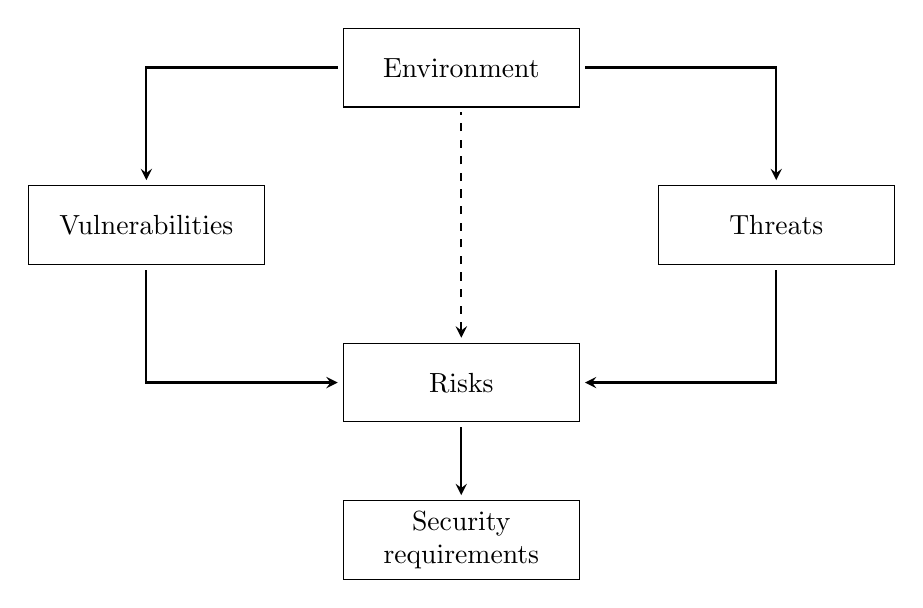
\begin{tikzpicture}[
    arrow/.style={thick,<-,shorten >=2pt,shorten <=2pt,>=stealth},
]
    \draw (4,6) rectangle (7,7) node [pos=.5] {Environment};
    \draw (0,4) rectangle (3,5) node [pos=.5,align=center] {Vulnerabilities};
    \draw (8,4) rectangle (11,5) node [pos=.5] {Threats};
    \draw (4,2) rectangle (7,3) node [pos=.5] {Risks};
    \draw (4,0) rectangle (7,1) node [pos=.5,align=center] {Security\\requirements};

    \draw[arrow] (1.5,5) -- (1.5,6.5) -- (4,6.5);
    \draw[arrow] (9.5,5) -- (9.5,6.5) -- (7,6.5);

    \draw[arrow] (4,2.5) -- (1.5,2.5) -- (1.5,4);
    \draw[arrow] (7,2.5) -- (9.5,2.5) -- (9.5,4);

    \draw[arrow,dashed] (5.5,3) -- (5.5,6);
    \draw[arrow] (5.5,1) -- (5.5,2);
\end{tikzpicture}

    %    }
    %    \caption{EBIOS method}
    %\end{figure}
\end{frame}

\begin{frame}
    \frametitle{Specification of Attack Scenarios}

    \begin{figure}[htb]
        \resizebox{.35\textwidth}{!}{
            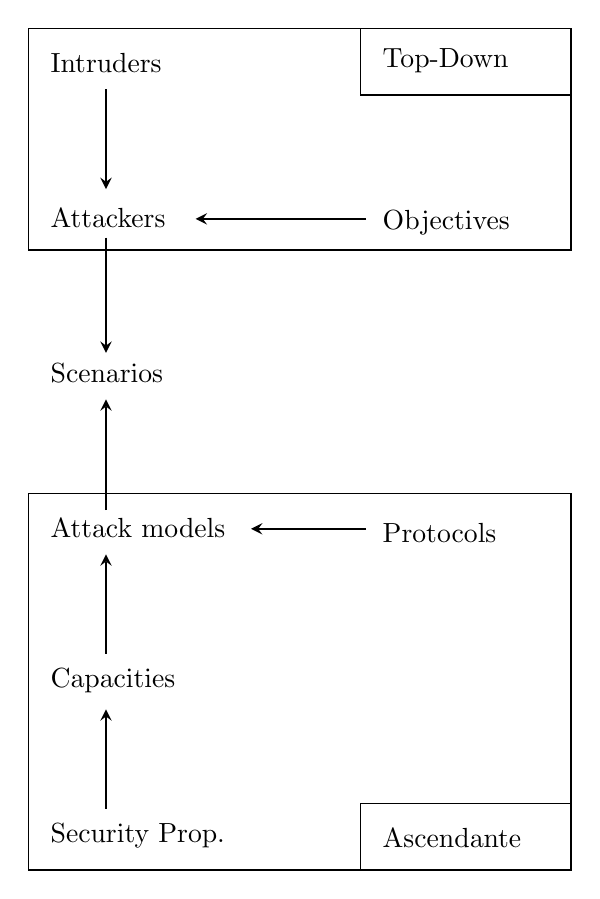
\begin{tikzpicture}[y=0.80pt, x=0.80pt, yscale=-1.000000, xscale=1.000000, inner sep=0pt, outer sep=0pt,
        arrow/.style={thick,->,shorten >=2pt,shorten <=2pt,>=stealth},
    ]
    \path[draw=black,miter limit=4.00,line width=0.600pt,rounded corners=0.0000cm] (40,40)  rectangle (285,140);
    \path[draw=black,miter limit=4.00,line width=0.600pt,rounded corners=0.0000cm] (190,40) rectangle (285,70);

    \path[fill=black] (50,60)   node[above right] (text2987) {Intruders};
    \path[fill=black] (200,60)  node[above right] (text2991) {Top-Down};
    \path[fill=black] (50,130)  node[above right] (text2995) {Attackers};
    \path[fill=black] (200,133) node[above right] (text2999) {Objectives};


    \draw[arrow] (75,65) -- (75,115) node {};
    \draw[arrow] (195,126) -- (113,126) node {};

    \draw[arrow] (75,132) -- (75,189) node {};
    \path[fill=black] (50,200) node[above right] (text3005) {Scenarios};
    \draw[arrow] (75,260) -- (75,205) node {};

    \path[draw=black,miter limit=4.00,line width=0.600pt,rounded corners=0.0000cm] (40,250)  rectangle (285,420);
    \path[draw=black,miter limit=4.00,line width=0.600pt,rounded corners=0.0000cm] (190,390) rectangle (285,420);

    \path[fill=black] (50,270)  node[above right] (text3023) {Attack models};
    \path[fill=black] (50,340)  node[above right] (text3009) {Capacities};
    \path[fill=black] (50,410)  node[above right] (text3019) {Security Prop.};
    \path[fill=black] (200,272) node[above right] (text3013) {Protocols};
    \path[fill=black] (200,410) node[above right] (text3029) {Ascendante};

    \draw[arrow] (75,325)  -- (75,275)  node {};
    \draw[arrow] (75,395)  -- (75,345)  node {};
    \draw[arrow] (195,266) -- (138,266) node {};
\end{tikzpicture}

        }
        \caption{Attack specification}
    \end{figure}
\end{frame}

\begin{frame}
    \frametitle{A Simple Example}

    \vspace{-.7em}
    \begin{figure}[htb]
        \resizebox{.7\textwidth}{!}{
            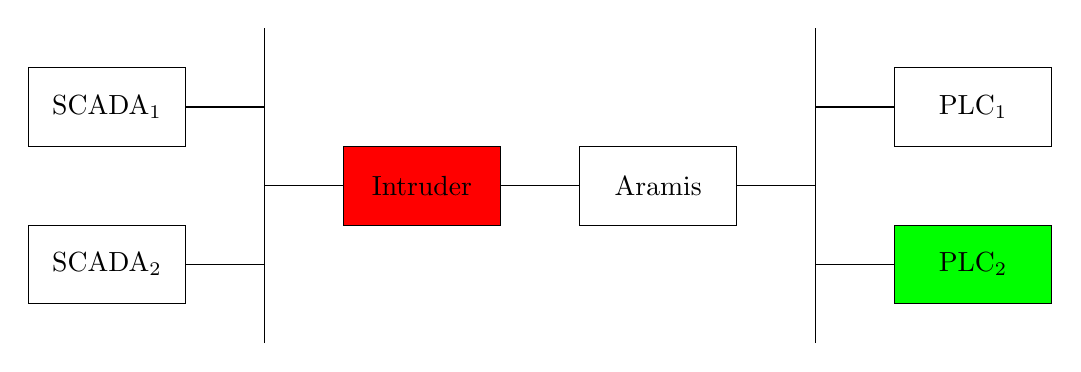
\begin{tikzpicture}[
        typetag/.style={rectangle, draw}
    ]
    %\draw [help lines] (0,0) grid (10,10);

    \draw (0,1) rectangle (2,2) node [pos=.5] {SCADA$_{2}$}; 
    \draw (0,3) rectangle (2,4) node [pos=.5] {SCADA$_{1}$}; 

    \draw (2,1.5) -- (3,1.5);
    \draw (2,3.5) -- (3,3.5);
    
    \draw (3,.5) -- (3,4.5);

    \draw (3,2.5) -- (4,2.5);
    \draw[fill=red] (4,2) rectangle (6,3) node [pos=.5] {Intruder};

    \draw (6,2.5) -- (7,2.5);
    \draw (7,2) rectangle (9,3) node [pos=.5] {\aramis};
    \draw (9,2.5) -- (10,2.5);

    \draw (10,.5) -- (10,4.5);

    \draw (10,1.5) -- (11,1.5);
    \draw (10,3.5) -- (11,3.5);
    
    \draw[fill=green] (11,1) rectangle (13,2) node [pos=.5] {PLC$_{2}$}; 
    \draw (11,3) rectangle (13,4) node [pos=.5] {PLC$_{1}$}; 
\end{tikzpicture}

        }
        \caption{Network architecture}
    \end{figure}
    \vspace{-1em}
    \begin{itemize}
        \item Objective of {\color{red} Intruder}: Attack the integrity of the comm. to {\color{green!70!black} PLC$_{2}$}.
        \begin{itemize}
            \item Realization: message replay, modification, ...
        \end{itemize}
            \vfill
        \item Protocol of {\color{green!70!black} PLC$_{2}$}: \opcua (2 security modes).
            \vfill
        \item Capacities of {\color{red} Intruder}:
        \begin{itemize}
            \item None if secured mode.
            \item Replay and forge if not secured mode.
        \end{itemize}
            \vfill
        \item Attack scenario: {\color{red} Intruder} replays a request on unsecure \opcua.
    \end{itemize}
\end{frame}

\begin{frame}
    \frametitle{General Approach}

    \vspace{-2em}
    \begin{figure}[htb]
        \resizebox{\textwidth}{!}{
            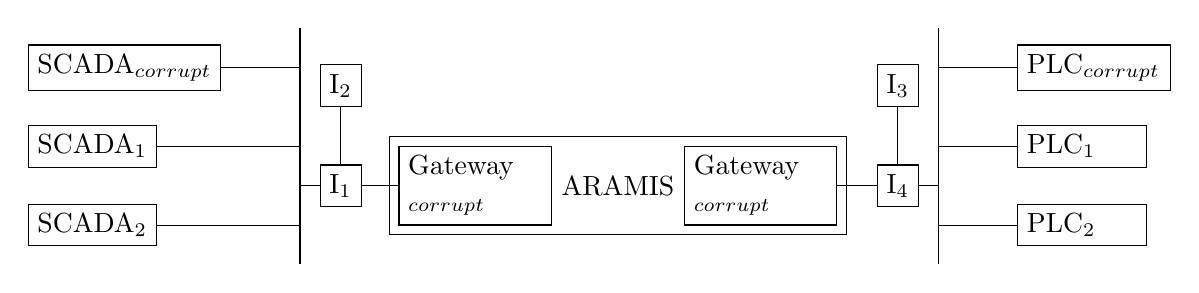
\begin{tikzpicture}[
        typetag/.style={rectangle, draw}
    ]
    \node[draw, anchor=west] (SCADA2) at (0,0.5){SCADA$_{2}$}; 
    \node[draw, anchor=west] (SCADA1) at (0,1.5){SCADA$_{1}$}; 
    \node[draw, anchor=west] (SCADAc) at (0,2.5){SCADA$_{corrupt}$};
    
    \coordinate (bus0) at ($(1,0)+(SCADAc.east |- 42,0)$);
    \draw (bus0) -- (bus0 |- 42,3);

    \draw (SCADA2.east) -- (bus0 |- SCADA2.east);
    \draw (SCADA1.east) -- (bus0 |- SCADA1.east);
    \draw (SCADAc.east) -- (bus0 |- SCADAc.east);

    \node[draw, anchor=west] (I1) at ($(0.25,0)+(bus0 |- 42,1)$){I$_{1}$};

    \node[anchor=west, typetag, text width=1.7cm] (GHc) at ($(1.25,0)+(bus0 |- 42,1)$) {Gateway\\$_{corrupt}$};
    \node[anchor=west] (ARAMIS) at (GHc.east){ARAMIS};
    \node[anchor=west, typetag, text width=1.7cm] (GBc) at (ARAMIS.east) {Gateway\\$_{corrupt}$};
    \node[draw, fit={(ARAMIS) (GHc) (GBc)}] {};

    \draw (bus0 |- I1.west) -- (I1.west);
    \draw (I1.east) -- (GHc.west);

    \node[draw] (I2) at ($(I1.north)+(0,1)$){I$_{2}$};
    \draw (I2.south) -- (I1.north);
    
    \node[draw, anchor=west] (I4) at ($(0.5,0)+(GBc.east |- 42,1)$){I$_{4}$};
    
    \coordinate (bus1) at ($(0.25,0)+(I4.east |- 42,0)$);
    \draw (bus1) -- (bus1 |- 42,3);

    \draw (GBc.east) -- (I4.west);

    \node[draw] (I3) at ($(I4.north)+(0,1)$){I$_{3}$};
    \draw (I3.south) -- (I4.north);

    \node[draw, anchor=west, text width=1.4cm] (PLC2) at ($(1,0)+(bus1 |- 42,0.5)$){PLC$_{2}$};
    \node[draw, anchor=west, text width=1.4cm] (PLC1) at ($(1,0)+(bus1 |- 42,1.5)$){PLC$_{1}$};
    \node[draw, anchor=west, text width=1.7cm] (PLCc) at ($(1,0)+(bus1 |- 42,2.5)$){PLC$_{corrupt}$};
    
    \draw (I4.east) -- (bus1 |- I4.east);
    \draw (PLC2.west) -- (bus1 |- PLC2.west);
    \draw (PLC1.west) -- (bus1 |- PLC1.west);
    \draw (PLCc.west) -- (bus1 |- PLCc.west);
\end{tikzpicture}

        }
        \caption{Network architecture}
    \end{figure}
    \vfill
    \begin{itemize}
        \item Systematic study of multiple possible parameters:
        \begin{itemize}
            \item Attackers, objectives, protocoles, capacities, ...
        \end{itemize}
        %\item More than one attacker (possibly colluding).
        %\item More complex objectives.
        %\item More capacities than forging.
        %\item Several protocols with different security properties
        %\begin{itemize}
        %    \item And different security modes.
        %\end{itemize}
        %    \vfill
        %\item Perspective: Interference of flows within ARAMIS device.
    \end{itemize}
\end{frame}

\begin{frame}
    \frametitle{Attack Traffic Generation}

    \begin{itemize}
        \item From scenarios of attack models.
    \end{itemize}
    \vfill
    \begin{figure}[htb]
        \resizebox{.8\textwidth}{!}{
            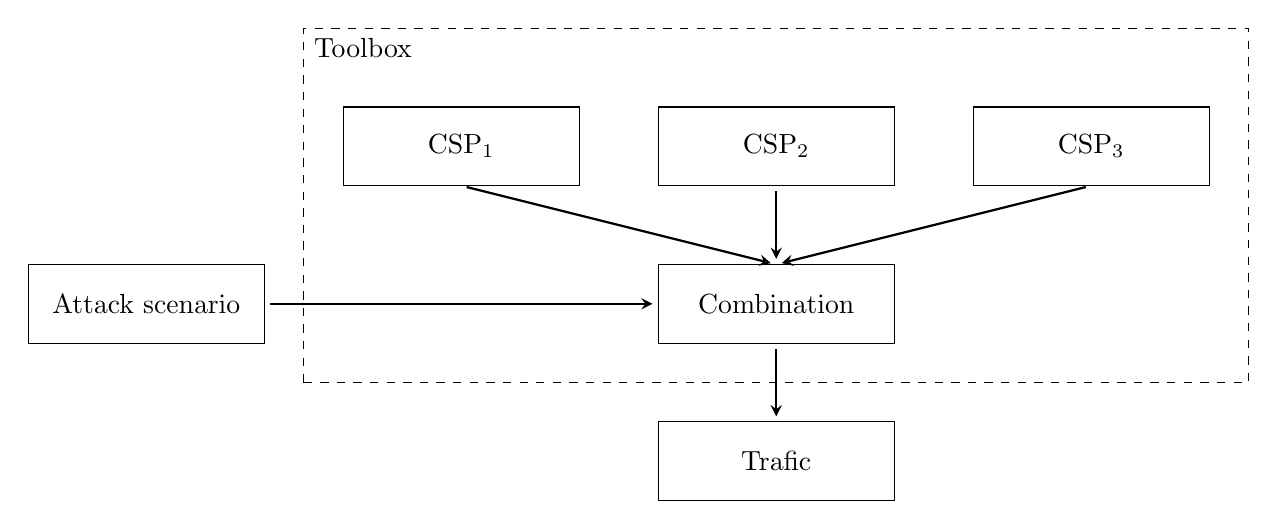
\begin{tikzpicture}[
    arrow/.style={thick,<-,shorten >=2pt,shorten <=2pt,>=stealth},
]
    \draw[dashed] (-.5,1.5) rectangle (11.5,6) node at (.25,5.75) {Toolbox};
    
    \draw (0,4) rectangle (3,5) node [pos=.5] {CSP$_1$};
    \draw (4,4) rectangle (7,5) node [pos=.5] {CSP$_2$};
    \draw (8,4) rectangle (11,5) node [pos=.5] {CSP$_3$};

    \draw (-4,2) rectangle (-1,3) node [pos=.5] {Attack scenario};
    \draw (4,2) rectangle (7,3) node [pos=.5] {Combination};

    \draw (4,0) rectangle (7,1) node [pos=.5] {Trafic};

    \draw[arrow] (4,2.5) -- (-1,2.5);

    \draw[arrow] (5.5,3) -- (1.5,4);
    \draw[arrow] (5.5,3) -- (5.5,4);
    \draw[arrow] (5.5,3) -- (9.5,4);

    %\draw[arrow] (1.5,1) -- (1.5,2);
    \draw[arrow] (5.5,1) -- (5.5,2);
    %\draw[arrow] (9.5,1) -- (9.5,2);
\end{tikzpicture}

        }
        \caption{How to generate attack traffic}
    \end{figure}
    \vfill
    \begin{itemize}
        \item Supervision of two TER interns with Emmanuel Perrier:
        \begin{itemize}
            \item Francesco Furfaro and Joris Chaffard.
        \end{itemize}
    \end{itemize}
\end{frame}

%\begin{frame}[fragile]
%    \frametitle{CSP\cite{Hoa78} Example}
%
%    \begin{itemize}
%        \item Replay a message
%    \end{itemize}
%    \vfill
%    \begin{lstlisting}[caption=Pseudo CSP for message replay]
%P() =
%    c?packet ->
%    RemoveHeader(packet, msg) ->
%    c!msg ->
%    STOP
%    \end{lstlisting}
%    \vfill
%    \begin{itemize}
%        \item RemoveHeader() is another helper (possibly not in CSP).
%    \end{itemize}
%\end{frame}

\section{Verification of Industrial Protocols}

\begin{frame}
    \frametitle{Table of Contents}
    
    \tableofcontents[currentsection]
\end{frame}

\begin{frame}
    \frametitle{Cryptographic Protocol Verification}

    \begin{itemize}
        \item Attack modeling relies on security properties of protocols.
        \begin{itemize}
            \item Check if they are ensured.
        \end{itemize}
            \vfill
        \item How to use protocol verification tools (e.g.: AVISPA\cite{AVISPA06_manual}, ProVerif\cite{Bla01}) on industrial protocols?
        \begin{itemize}
            \item Tools can verify secrecy and authentication.
        \end{itemize}
            \vfill
        \item Focus on properties required by industry:
        \begin{itemize}
            \item Integrity.
            \item Availability.
        \end{itemize}
    \end{itemize}
    %\vfill
    %\begin{block}{Flow integrity}
    %    Messages received by a peer are the same as those sent by another.
    %    
    %    Take into account the order of the messages.
    %\end{block}
\end{frame}

\begin{frame}
    \frametitle{Modeling \opcua}

    \begin{itemize}
        \item New standard for industrial communications.
        \item Security similar to TLS\cite{DR08}.
    \end{itemize}
    \begin{columns}
        \begin{column}{.5\textwidth}
            \begin{figure}[htb]
                \resizebox{1.1\textwidth}{!}{
                    \includegraphics{opcua}
                }
                \caption{Sub-protocol of \opcua}
            \end{figure}
        \end{column}
        \begin{column}{.5\textwidth}
            \begin{itemize}
                \item Goal: Model \opcua in verification tools.
                \begin{enumerate}
                    \item Verify secrecy and authentication.
                    \item Model industry properties such as integrity.
                    \item Application to other industrial protocols.
                \end{enumerate}
            \end{itemize}
        \end{column}
    \end{columns}
\end{frame}

\begin{frame}
    \frametitle{Advanced modeling researches}

    \begin{block}{Benchmark of Verification Tools}
        \begin{itemize}
            \item Joint work with Pascal Lafourcade.
            \item Goal: Compare performances of some tools with complex algebraic properties.
            \begin{itemize}
                \item 6 tools compared on 21 protocols (nearly 400 test runs).
            \end{itemize}
            \item Publication in FPS'15.
        \end{itemize}
    \end{block}
    \vfill
    \begin{block}{Distributed Computation Protocol}
        \begin{itemize}
            \item Joint work with Pascal Lafourcade, Jean-Guillaume Dumas (LJK) and Jean-Baptiste Orfila (LJK).
            \item Goal: Prove the security of a distributed computation protocol.
            \begin{itemize}
                \item New algebraic properties: Homomorphic properties.
            \end{itemize}
            %\item Submitted to AFRICACRYPT'16.
        \end{itemize}
    \end{block}
    %\begin{itemize}
    %    \item Interest for the thesis: Advanced aspects of the verification tools.
    %\end{itemize}
\end{frame}

\begin{frame}
    \frametitle{Conclusion}

    \begin{figure}[htb]
        \centering
        \resizebox {.7\textwidth} {!} {
            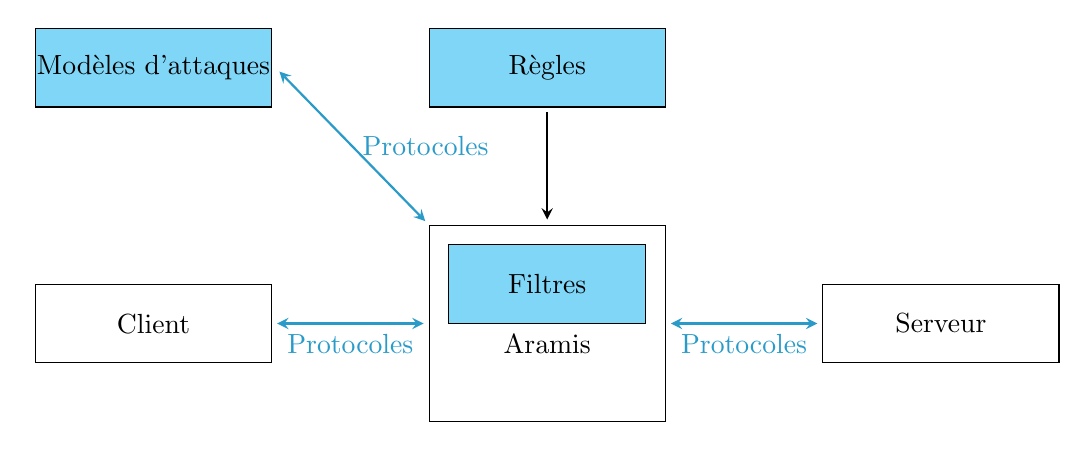
\begin{tikzpicture}[
    arrow/.style={thick,->,shorten >=2pt,shorten <=2pt,>=stealth},
    darrow/.style={thick,<->,shorten >=2pt,shorten <=2pt,>=stealth},
]

    \draw (0,.75) rectangle (3,1.75) node [pos=.5] {Client};
    
    %\fill[cyan!50!white] (5,0) rectangle (8,2.5);
    \draw (5,0) rectangle (8,2.5) node [pos=.5,below=.4] {\aramis};
    \fill[cyan!50!white] (5.25,1.25) rectangle (7.75,2.25);
    \draw (5.25,1.25) rectangle (7.75,2.25) node [pos=.5] {Filtres};
    
    \draw (10,.75) rectangle (13,1.75) node [pos=.5] {Serveur};

    \fill[cyan!50!white] (0,4) rectangle (3,5);
    \draw (0,4) rectangle (3,5) node [pos=.5] {Modèles d'attaques};

    \draw[darrow,cyan!80!black] (3.05,4.5) -- (5,2.5) node [pos=.5,right] {Protocoles};

    \fill[cyan!50!white] (5,4) rectangle (8,5);
    \draw (5,4) rectangle (8,5) node [pos=.5] {Règles};

    \draw[arrow,] (6.5,4) -- (6.5,2.5);

    \draw[darrow,cyan!80!black] (3,1.25) -- (5,1.25) node [pos=.5,below] {Protocoles};
    \draw[darrow,cyan!80!black] (8,1.25) -- (10,1.25) node [pos=.5,below] {Protocoles};

    %\draw[dashed,cyan!80!black] (-.25,-.25) rectangle (13.25,5.25);
    %\draw node [align=left,below right,cyan!80!black] at (0,5) {{\bf Attack models}};
    %\draw node [align=left,below right,cyan!80!black] at (0,4.5) {Produce attack\\scenarios given\\a system and\\attacker objectives};
\end{tikzpicture}

        }
        \caption{Axes of my thesis}
    \end{figure}
    \vspace{-1em}
    \begin{itemize}
        \item Strong industrial context.
        \item Stimulating interaction with government agencies.
        \item Possible project with LIG and GIPSA-lab on attack generation against industrial systems.
    \end{itemize}
\end{frame}

\begin{frame}
    \frametitle{Complete Publication List}

    \begin{enumerate}
        \item M. Potet, L. Mounier, M. Puys, and L. Dureuil. {\bf Lazart: A symbolic approach for evaluation the robustness of secured codes against control Flow Injections.} In {\em ICST'14}, 2014.
            \vfill
        \item M. Puys, L. Rivi\`ere, J. Bringer, and T. Le. {\bf High-Level Simulation for multiple fault Injection Evaluation.} In {\em QASA'14}, 2014.
            \vfill
        \item L. Rivi\`ere, M. Potet, T. Le, J. Bringer, H. Chabanne, and M. Puys. {\bf Combining High-Level and low-level approaches to evaluate software implementations robustness against multiple fault Injection Attacks.} In {\em FPS'14}, 2014.
            \vfill
        \item P. Lafourcade and M. Puys. {\bf Performance Evaluations of cryptographic protocols verification tools dealing with Algebraic Properties.} In {\em FPS'15}, 2015.
    \end{enumerate}
\end{frame}

\begin{frame}
    \frametitle{Conclusion}

    \begin{center}
        Thanks for your attention!
    \end{center}
\end{frame}

\begin{frame}
    \frametitle{Safety and Security}
    
    \begin{figure}[htb]
        \resizebox{.6\columnwidth}{!}{
            %\includegraphics{liens_safety_secu}
            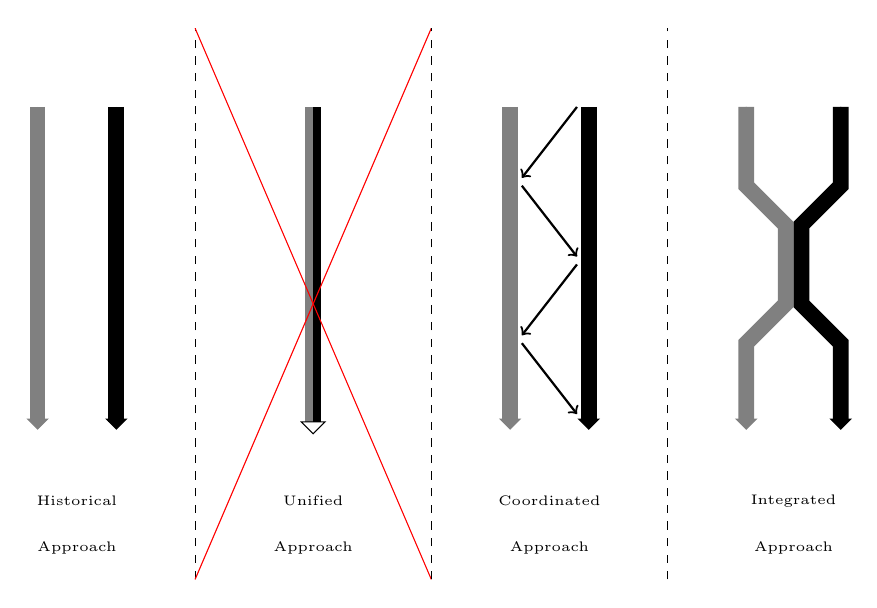
\begin{tikzpicture}[
    myarrow/.style={
        draw=black,solid,line width=2mm, postaction={-triangle 90,thin,draw,shorten >=-1mm}
}]
    %\draw[->, very thick] (0,0) -- (0,-1) -- (1,-1.5) -- (1,-2.5) -- (0,-3);
    \path[myarrow, gray] (0,5) -- (0,1);
    \path[myarrow] (1,5) -- (1,1);
    \draw node [align=center] at (.5,0) {\tiny Historical};
    \draw node [align=center] at (.5,-.6) {\tiny Approach};

    \draw[dashed] (2,-1) -- (2,6);

    \fill[gray] (3.4,1) rectangle (3.5,5);
    \fill[black] (3.5,1) rectangle (3.6,5);
    \draw (3.35,1) -- (3.65,1) -- (3.5,.85) -- cycle;
    \draw node [align=center] at (3.5,0) {\tiny Unified};
    \draw node [align=center] at (3.5,-.6) {\tiny Approach};

    \draw[red] (2,-1) -- (5,6);
    \draw[red] (5,-1) -- (2,6);

    \draw[dashed] (5,-1) -- (5,6);
    
    \path[myarrow, gray] (6,5) -- (6,1);
    \path[myarrow] (7,5) -- (7,1);
    \draw[->,thick] (6.85,5) -- (6.15,4.1);
    \draw[->,thick] (6.15,4) -- (6.85,3.1);
    \draw[->,thick] (6.85,3) -- (6.15,2.1);
    \draw[->,thick] (6.15,2) -- (6.85,1.1);
    \draw node [align=center] at (6.5,0) {\tiny Coordinated};
    \draw node [align=center] at (6.5,-.6) {\tiny Approach};

    \draw[dashed] (8,-1) -- (8,6);
    
    \path[myarrow, gray] (9,5) -- (9,4) -- (9.5,3.5) -- (9.5,2.5) -- (9,2) -- (9,1);
    \path[myarrow] (10.2,5) -- (10.2,4) -- (9.7,3.5) -- (9.7,2.5) -- (10.2,2) -- (10.2,1);
    \draw node [align=center] at (9.6,0) {\tiny Integrated};
    \draw node [align=center] at (9.6,-.6) {\tiny Approach};
\end{tikzpicture}

        }
        \caption{How to link safety and security \cite{Pie10}}
    \end{figure}
\end{frame}

\begin{frame}
    \frametitle{Purdue Model}

    \begin{figure}[htb]
        \resizebox{.8\columnwidth}{!}{
            \def\levelPhy{\small 0. Physical process}
\def\levelAut{\small 1. Automata controling the process}
\def\levelSup{\small 2. SCADA: supervision and control}
\def\levelOpp{\small 3. Production management}
\def\levelBus{\small 4. Business level, classical IT}

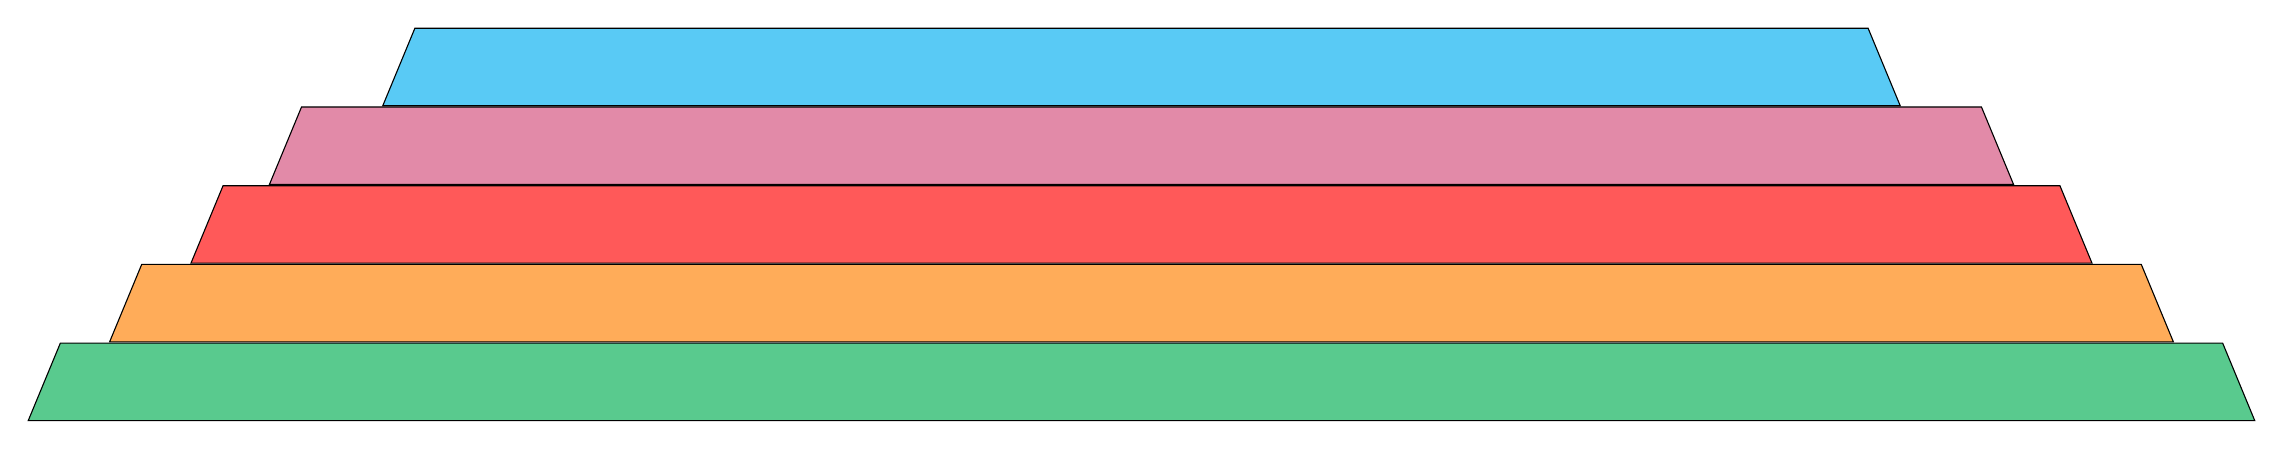
\begin{tikzpicture}[
    mytrap/.style={
    trapezium, trapezium angle=67.5, draw,inner xsep=0,outer sep=0,
    minimum height=28, text width=#1,align=center
}]

\begin{scope}[fill opacity=0.65]
        \foreach \ancho/\T/\C [count=\xi] in {186/\levelPhy/green!68!blue,172/\levelAut/orange,158/\levelSup/red,144.5/\levelOpp/purple!70,125/\levelBus/cyan}
            \node [mytrap=\ancho,fill=\C] at (0,\xi) [text opacity=1] {\T};
    \end{scope}
\end{tikzpicture}

        }

        \caption{Purdue model \cite{Wil91}}
    \end{figure}
\end{frame}

\begin{frame}
    \frametitle{Cryptograpfic Protocols Verification}

    \begin{exampleblock}{Needham-Schroeder}
        \vspace{-.8em}
        \begin{columns}
            \begin{column}{.45\textwidth}
            \begin{enumerate}
                \item A $\rightarrow$ B : $\{A,N_{A}\}_{KB}$
                \item B $\rightarrow$ A : $\{N_{A},N_{B}\}_{KA}$
                \item A $\rightarrow$ B : $\{N_{B}\}_{KB}$
            \end{enumerate}
            \end{column}
            ~
            \begin{column}{.45\textwidth}
                Designed and {\bf proved} in 1978.\\% by Roger Needham and Michael Schroeder.\\
                Broken in 1996 (17 years after).\\% by Gavin Lowe using \casperfdr, known as {\em Man-In-The-Middle} attack.\\
            \end{column}
        \end{columns}
    \end{exampleblock}

    \begin{exampleblock}{Man-In-The-Middle attack}
        \vspace{-.8em}
        \begin{columns}
            \begin{column}{.45\textwidth}
                \begin{enumerate}
                    \item A $\rightarrow$ I : $\{A,N_{A}\}_{KI}$
                    \item[]
                    \item[]
                          \setcounter{enumi}{1}
                    \item I $\rightarrow$ A : $\{N_{A},N_{B}\}_{KA}$
                    \item A $\rightarrow$ I : $\{N_{B}\}_{KI}$
                    \item[]
                \end{enumerate}
            \end{column}
            ~
            \begin{column}{.45\textwidth}
                \begin{enumerate}
                    \item[]
                          \setcounter{enumi}{0}
                    \item I $\rightarrow$ B : $\{A,N_{A}\}_{KB}$
                    \item B $\rightarrow$ I : $\{N_{A},N_{B}\}_{KA}$
                    \item[]
                    \item[]
                          \setcounter{enumi}{2}
                    \item I $\rightarrow$ B : $\{N_{B}\}_{KB}$
                \end{enumerate}
            \end{column}
        \end{columns}
    \end{exampleblock}
    \vfill
    \begin{itemize}
        \item Way too much possible combinations.% outpaces the humans' capabilities.
        \begin{itemize}
            \item Need of automation using tools.
        \end{itemize}
    \end{itemize}
\end{frame}

\begin{frame}[allowframebreaks]
    \frametitle{References}
    
    \bibliographystyle{amsalpha}
    \bibliography{phdBiblio}
\end{frame}

\end{document}
